\documentclass[11pt]{beamer}
\definecolor{spoiler}{gray}{0.6}

\usepackage[utf8x]{inputenc}
\usepackage[T2A]{fontenc}
\usepackage[russian]{babel}
\usepackage{xcolor}
\usepackage{MnSymbol}
\usepackage{mathrsfs}
\usepackage{listings}
\usepackage{mathtools}
\usepackage{amssymb,amsmath, dsfont, amsthm}
\usepackage{hyperref}
\hypersetup{unicode=true}
\usepackage{comment}
\usepackage{graphicx}
\usepackage{tikz,makecell}
\usepackage{wrapfig}
\usepackage{xfrac}
\usepackage{qrcode}

\usetheme{Berlin}

\usecolortheme{dolphin}
\title[Петербургский Турнир и Регата]
	{\bfseries Петербургский Турнир и Регата}
\author[Тодоров Е.И.]{Тодоров Е.И.}
\institute{Санкт-Петербургский Турнир юных математиков, Фонд <<Время науки>>}
\date{\today}

\newtheorem{Th}{Теорема}
\newtheorem{Def}{Определение}
\newtheorem{Ex}{Пример}
\newtheorem{Proposition}{Предложения}
\newtheorem{Property}{Свойство}
\newtheorem{Prof}{Доказательство}
\newtheorem{Profcont}{Доказательство (продолжение)}

\newcommand\fram[2]{\begin{frame}{\bf #1} #2 \end{frame}}
\newcommand{\comm}[1]{$\backslash$\texttt{#1}}
\def\scolon{\rlap{,}\raisebox{0.8ex}{,} }
\def\mitem{\medskip\item}
\newcommand{\myref}[2]{\href{#1}{\texttt{\underline{#2}}}}
\newcommand{\set}[1]{\left\{ #1 \right\}}

\def\usl#1#2{\begin{block}{#1} #2 \end{block} \medskip\pause}
\def\uslnp#1#2{\begin{block}{#1} #2 \end{block} \medskip}

\newcommand{\hackcenter}[1]{
 \xy (0,0)*{#1}; \endxy}
\newcommand{\scs}{\scriptstyle}
\newcommand{\xsum}[2]{
 \xy
 (0,.4)*{\sum};
 (0,3.7)*{\scs #2};
 (0,-2.9)*{\scs #1};
 \endxy
}
\newcommand{\refequal}[1]{\xy {\ar@{=}^{#1}
(-1,0)*{};(1,0)*{}};
\endxy}

\usepackage[linguistics]{forest}

\newcommand{\fstfor}[5]{
	\begin{figure}[h] \centering
	\begin{forest} for tree={circle, draw, minimum size=1.7ex, inner sep=0.45pt,% 
	   l=#2cm, s sep=#3mm}
		#1
	\end{forest}
		\caption{#4} \label{#5}
	\end{figure}}


\begin{document}
\section{ }
\begin{frame}\titlepage\end{frame}

\fram{Эта презентация онлайн}{
\Large
\begin{center}
Зачем фотографировать презентацию, \\
		когда её можно скачать? \\[0.3cm]
		\qrcode[height=5cm]{http://bit.ly/TYM_pres}
\end{center}
}

\section{ТЮМы}
\fram{Краткая история ТЮМов}{
\Large
\begin{itemize}
	\item формат подглядели у ТЮФов;\vspace{2mm}
	\item было и есть много турниров мат.боёв;\vspace{2mm}
	\item 1999 --- первый РТЮМ;\vspace{2mm}
	\item 2009 --- первый ITYM;\vspace{2mm}
	\item 2013 --- первый СПбТЮМ.
\end{itemize}
}

\section{Что такое ТЮМ?}
\fram{Особенности ТЮМов}{
\large
\begin{itemize}
	\item исследовательский характер задач;\vspace{2mm}
	\item задачи решаются дома, на это даётся 1.5--2.5 месяца;\vspace{2mm}
	\item жеребьёвки и перетягивания;\vspace{2mm}
	\item в одном бою участвует не 2, а 3--5 команд;\vspace{2mm}
	\item больше разных ролей (4 типа);\vspace{2mm}
	\item письменные рецензии;\vspace{2mm}
	\item зачастую, более квалифицированное жюри.
\end{itemize}
}

\fram{Докладчик}{
\Large
\begin{itemize}
\item оформляет письменное решение;\vspace{1mm}
\item делает презентацию;\vspace{1mm}
\item рассказывает основные результаты на бою;\vspace{1mm}
\item должен хорошо знать своё решение и теорию;\vspace{1mm}
\item ведёт дискуссию с Оппонентом и Рецензентом;\vspace{1mm}
\item отвечает на вопросы жюри;\vspace{1mm}
\item роль с максимальным возможным баллом.
\end{itemize}
}

\fram{Оппонент}{
\Large
\begin{itemize}
	\item оформляет письменную рецензию;\vspace{1mm}
	\item следит за докладом;\vspace{1mm}
	\item задаёт вопросы по решению и докладу;\vspace{1mm}
	\item указывает на ошибки и неточности;\vspace{1mm}
	\item должен хорошо знать решение \linebreak Докладчика  и теорию;\vspace{1mm}
	\item оценивает решение и доклад;\vspace{1mm}
	\item отвечает на вопросы Рецензента и жюри.
\end{itemize}
}

\fram{Рецензент}{
\Large
\begin{itemize}
	\item оформляет письменную рецензию;\vspace{1mm}
	\item следит~за~дискуссией~Докладчика~и~Оппонента;
	\item даёт оценку дискуссии;
	\item задаёт вопросы Оппоненту, \linebreak проверяет понимание;
	\item указывает на ошибки, упущенные Оппонентом;
	\item должен внимательно следить за дискуссией;
	\item должен хорошо знать решение \linebreak Докладчика  и теорию;
	\item отвечает на вопросы жюри.
\end{itemize}
}

\fram{Наблюдатель}{
\Large
\begin{itemize}
	\item оформляет письменную рецензию;
	\item внимательно следит за ходом \linebreak доклада и дискуссий;
	\item выходит только если никто не заметил серьёзную ошибку;
	\item должен хорошо знать решение \linebreak Докладчика  и теорию;
	\item в случае выхода отвечает на вопросы жюри;
	\item может получить отрицательные баллы за неуместное выступление.
\end{itemize}
}

\section{СПбТЮМ}
\fram{История Петербургского Турнира}{
\large

\begin{itemize}
	\item в 2013 начался, как проект \myref{https://lnmo.ru/}{ЛНМО};
	\item с 2015 является проектом \myref{https://timeforscience.ru/}{Фонда <<Время науки>>};
	\item в 2018 появтяется Турнир младшей лиги;
	\item летом 2020 впервые проводится онлайн;
	\item в 2020 появляется математическая Регата;
	\item команды из сильнейших математических школ России, Беларуси, Донецка;
	\item Турнир Младшей возрастной группы в 2020 году \linebreak собрал 32 команды.
\end{itemize}
}

\section{Задачи Турнира} %особенности и примеры
\fram{Избранные задачи Турнира}{
\usl{мл.-2020-Ник Николс-1-(b)}{
Сколько палочек может понадобиться Кате, чтобы сложить клетчатый прямоугольник, состоящий из 4; 8; 30 клеточек?
}

\begin{itemize}
	\item 12, 13;
	\item 22, 25;
	\item 71, 73, 77, 91.
\end{itemize}
}

\fram{}{
\usl{мл.-2020-Ник Николс-2-(b)}{
Пусть известно, что на то, чтобы собрать некоторый клетчатый прямоугольник, Кате понадобилось $17$; $19$; $22$; $24$; $52$ палочки. Сколько клеточек могло быть в таком прямоугольнике? Интерес представляет поиск всевозможных вариантов и выявление закономерностей.
}

\begin{itemize}
	\item $2 \times 3$;
	\item $1 \times 6$;
	\item $1 \times 7$, $2 \times 4$;
	\item $3 \times 3$;
	\item $1 \times 17$, $2 \times 10$, $3 \times 7$.
\end{itemize}
}

\fram{}{
\uslnp{мл.-2019-Лазерное шоу-1}{
Разместим плоские зеркала, которые на плоскости будем отмечать отрезками. Разрешим лучу отражаться от одного зеркала лишь в одной точке.
\begin{enumerate}
\item[(a)] Докажите, что наибольшее число отражений, которое может сделать луч в системе из
двух зеркал, равно трём. Опишите все такие системы зеркал.
\item[(b)] Докажите, что наибольшее число отражений, которое может сделать луч в системе из
трёх зеркал, равно семи. Опишите все такие системы зеркал.
\end{enumerate}
}
}

\section{Регата}
\fram{Регата}{
\Large

\begin{itemize}
	\item нестандартные задачи;
	\item готовят к формату Турнира;
	\item 3 серии по 3--4 задачи;
	\item на решение даётся по 1,5--2 дня;
	\item решения сдаются дистанционно и письменно;
	\item решения проверяют авторы задач.
\end{itemize}
}

\section{Задачи Регаты}
\fram{Избранные задачи Регаты}{
\uslnp{ст.-2020-Игры с карточками-2}{
Каждый из автоматов принимает карточки и выдаёт взамен новые, числа на которых определяются по закону, которому подчиняется данный автомат. Пусть первый автомат выдаёт по карточке с числом $x$ карточку с числом $x+1$, второй автомат по карточке с числом $x$ выдаёт карточку с числом $\frac{-x}{2}$.
\begin{enumerate}
	\item У вас имеется лишь карточка с числом 0. Ответьте на следующие вопросы:
	\begin{enumerate}
		\item Как с помощью рабочих автоматов получить карточку с числом −10?
		\item Как с помощью рабочих автоматов получить карточку с числом $\frac{3}{16}$?
		\item Возможно ли получить карточку с числом $\frac{1}{3}$?
	\end{enumerate}
\end{enumerate}
}
}

\fram{}{
\usl{мл.-2020-Растут вниз-1}{
Представим себе дерево, в котором все листья находятся на одной глубине, а все узлы имеют по три потомка. Счетовод Щоща хочет вписать в каждый узел дерева число, преобладающее среди трёх непосредственных потомков этого узла. Закончите работу Щощи на дереве на рисунке.
}\vspace{-4mm}
\begin{center}
	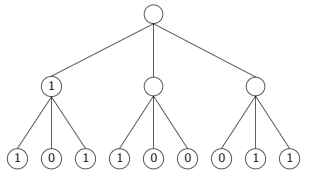
\includegraphics[width=6cm]{tree-1}
\end{center}
}

\fram{}{
\uslnp{мл.-2020-Растут вниз-2}{
Докажите, что любой пропущенный Щощей лист может значительно повлиять на ответ. А именно, для каждого из девяти листьев дерева глубины 2 постройте расстановку единиц инулей в остальные листья, такую, что при замене числа в выбранном листе меняется число,написанное в корне дерева.
}
}

\fram{}{
\ \vspace{-1cm}
\usl{мл.-2020-Взвешен и признан слишком лёгким}{
Во всей задаче мы будем рассматривать чашечные весы. Весы будут находиться в равновесии, если на всех чашах находится одинаковый вес. Взвесить $m$ килограмм на таких весах значить разложить гирьки таким образом, чтобы одна из чаш была тяжелее другой ровно на $m$ килограмм.
\begin{enumerate}
	\item Какие веса можно взвесить с помощью набора гирь весами в 2, 3 и 9 кг? А с помощью набора весами в 1, 3 и 9 кг?
	\item Докажите, что с помощью набора гирь в 1, 3, 9 и 27 кг можно взвесить любой вес, выражающийся натуральным числом от 1 до 40.
\end{enumerate}
}\vspace{-0.3cm}

\begin{itemize}
	\item $1,2,3,4,5,6,7,8,9,10,11,12,14$;
	\item $1,2,\ldots,13$.
\end{itemize}
}

\section{Присоединиться}
\fram{Собирай команду и вступай в бой!}{
\Large
\begin{center}
	Зарегистрировать команду на Регату:\vspace{0.2cm}
	
	\qrcode[height=5cm]{https://forms.gle/WuuC2qttGcfETTUm8} \vspace{0.2cm}
	
	(отсканируйте или тыкните на QR-код)
\end{center}
}

\section{ }
\fram{Математическая лекция}{
\Large
\begin{center}
	\qrcode[height=5cm]{http://bit.ly/lecture_sqrt2} \vspace{0.3cm}
%	\includegraphics[width=5cm]{sqrt2-link}
	
	(отсканируйте или тыкните на QR-код)
\end{center}
}

\fram{}{
\begin{center}\vspace{-2cm}
\begin{tabular}{lcr}
\makecell[c]{
\includegraphics[width=0.3\textwidth]{pgrants_logo.png}} &
\makecell[c]{
\includegraphics[width=0.3\textwidth]{TYM_logo.png}} &
\makecell[c]{
\includegraphics[width=0.3\textwidth]{fond_logo_hor}}
\end{tabular} \vspace{0.3cm}

    \large{Спасибо за внимание!} \vspace{0.5cm}
    
    Сайт Турнира: \myref{https://spbtym.ru/}{spbtym.ru} \vspace{1cm}
    
    Задать вопрос автору: \myref{mailto:todzhe@mail.ru}{todzhe@mail.ru}
\end{center}
}
\end{document}